\graphicspath{{fig/sim_studies/}}

\chapter{Simulation studies}
\label{cha:sim_studies}

The feasibility of performing parameter inference on real data can be assessed by
simulation study. In simulation studies, candidate models are forward simulated for known
parameter values. This simulated data is then used to verify that the known parameter
values can be recovered by inference.

If parameter inference is \emph{not} possible on simulated data, we know that the same
inference will not be possible on real data either. Simulation studies also provide a good
opportunity to assess (and frankly, debug) our implementation of MCMC algorithms
constructed to target the posterior distribution.

\section{Global models}
\label{sec:glob_mod}

Global models refer to models in which all agents take the \emph{same} parameter values.
These are in contrast to hierarchical models, in which all agents take \emph{different}
parameter values.  We shall first seek to perform simulation studies on global
models, as they represent a simpler inference problem.

Recall from Bayes' Theorem (\cref{eq:bayes_theorem}) that to realise the posterior
distribution we need to combine the likelihood of the data with our prior beliefs. Let us
begin by considering the likelihood of observing a single agent updating its direction, in
the presence of neighbours, from $\theta_{i, t}$ to $\theta_{i, t+1}$.  From
\cref{eq:students_update} we have that agent $i$ updates its direction as a draw from the
generalised Students $t$-distribution with location $\angmean{\theta}_{i,t}$, scale
$\sigma_Y$ and degrees of freedom $\nu$. As such, the likelihood of observing this
directional update can be quantified as:
\begin{equation*}
  L(\sigma_Y, \nu, \angmean{\theta}_{i,t} \given \theta_{i,t+1}) =
  \frac{\Gamma(\frac{\nu +1 }{2})}{\Gamma(\frac{\nu}{2})\sqrt{\pi\nu}\sigma_Y}
  \Bigg(1 + \frac{1}{\nu}
  \bigg(\frac{\theta_{i,t+1}-\angmean{\theta}_{i,t}}{\sigma_Y}\bigg)^2
  \Bigg)^{-\frac{\nu+1}{2}},
\end{equation*}
where $\Gamma$ is the gamma function. Building on this, let us consider the likelihood of
observing agent $i$'s directional updates from time $t$ to time $t+2$. As the noise
experienced by an agent is independent of the noise it experienced at previous time
steps, we may express this likelihood as a product
\begin{align*}
  L(\sigma_Y,\nu,\angmean{\theta}_{i,t},\angmean{\theta}_{i,t+1}\given\theta_{i,t+1},
  \theta_{i,t+2})
  = L(\sigma_Y,\nu,\angmean{\theta}_{i,t+1}\given\theta_{i,t+2})\times
  L(\sigma_Y,\nu,\angmean{\theta}_{i,t}\given\theta_{i,t+1}).
\end{align*}

In general, we wish to express the likelihood of observing agent $i$'s directional updates
over any number of times steps. Suppose then that we observe the directions of agent $i$
from time $t=1$ to time $t=T$. Again, as consecutive realisations from the noise
distribution are independent, we can compute the likelihood as a product
\begin{align*}
  L(\sigma_Y, \nu, \angmean{\theta}_{i,1:T-1} \given \theta_{i,2:T})
  = & \prod_{t=1}^{T-1} L(\sigma_Y,\nu,\angmean{\theta}_{i,t} \given \theta_{i,t+1}) \\
  = & \prod_{t=1}^{T-1}
  \frac{\Gamma(\frac{\nu +1 }{2})}{\Gamma(\frac{\nu}{2})\sqrt{\pi\nu}\sigma_Y}
  \Bigg(1 + \frac{1}{\nu}
  \bigg(\frac{\theta_{i,t+1}-\angmean{\theta}_{i,t}}{\sigma_Y}\bigg)^2
  \Bigg)^{-\frac{\nu+1}{2}},
\end{align*}
where $\angmean{\theta}_{i,1:T-1}$ is shorthand for
$\angmean{\theta}_{i,1},\angmean{\theta}_{i,2},\ldots,\angmean{\theta}_{i,T-1}$, and
similarly for $\theta_{i,2:T}$. Finally, although we have expressed the likelihood of
observing a single agent's directional changes over $T$ observations, we really wish to
express the likelihood of observing \emph{an entire flock's} directional changes over $T$
observations. Consider observing a flock of $N$ individuals over $T$ time steps. The
likelihood of observing their directional updates can be quantified as:
\begin{align}
  \label{eq:likelihood}
  \begin{split}
    L(\sigma_Y, \nu, \angmean{\theta}_{1:N,1:T-1} \given\theta_{1:N,2:T})
    &= \prod_{i=1}^N \prod_{t=1}^{T-1} L(\sigma_Y,\nu,\angmean{\theta}_{i,t}\given\theta_{i,t+1})  \\
    &= \prod_{i=1}^N \prod_{t=1}^{T-1}
    \frac{\Gamma(\frac{\nu +1 }{2})}{\Gamma(\frac{\nu}{2})\sqrt{\pi\nu}\sigma_Y}
    \Bigg(1 + \frac{1}{\nu}
    \bigg(\frac{\theta_{i,t+1}-\angmean{\theta}_{i,t}}{\sigma_Y}\bigg)^2
    \Bigg)^{-\frac{\nu+1}{2}}.
  \end{split}
\end{align}

The likelihood function for all our models takes the same form. What differs between
models is the specification of the weighting function $\omega_{ij,t}$ and the
corresponding computation of $\angmean{\theta}_{i,t}$.

\subsection{Vicsek model}

We simulate the Vicsek model to realise a flock of $N=45$ agents moving for $T=200$ time
steps. We desire to work with simulated data which is similar to real data. As such, the
initial conditions for this simulation are taken from an observation of a real flocking
event. Parameters $r=50$, $\sigma_Y=0.03$ and $\nu=7$ are set for this simulation.
\cref{fig:vicsek_sim_study} shows the data generated by this simulation. We seek to assess
whether we can recover the true parameter values from the simulated data.

\begin{figure}[tb]
  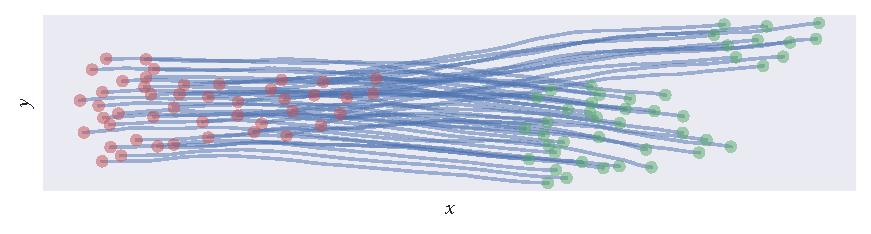
\includegraphics{vicsek_sim.pdf}
  \caption{The trajectories of $N=45$ agents simulated over $T=200$ time steps according to
    the Vicsek model. The initial conditions of the simulation reflect that of a real
    flocking event. The parameters of the model are given by $r=50$, $\sigma_Y=0.03$ and
    $\nu=7$.}
  \label{fig:vicsek_sim_study}
\end{figure}

The likelihood of observing the data can be quantified by \cref{eq:likelihood}. However,
to target the posterior we also need to specify our prior beliefs about the model
parameters. To allow the data to drive the inference, we shall specify weakly informative
priors. Once realisations from the posterior have been made, we overlay our priors to
assess how our beliefs have updated in light of the data.

Our prior beliefs about likely values for the degrees of freedom parameter $\nu$ shall be
reflected by a $\Ga(2, 0.1)$ distribution, as popularised by \textcite{juarez10}.  As $r$
and $\sigma_Y$ both represent strictly positive measures, we shall use a gamma
distribution to quantify our beliefs about them. These prior beliefs, as detailed in
\cref{eq:vicsek_priors} and visualised in \cref{fig:vicsek_priors}, represent vague
beliefs, allowing a large range of possible parameter values.
\begin{align}
  \label{eq:vicsek_priors}
  \begin{split}
    r           & \sim \Ga(50, 1) \\
    \sigma_Y    & \sim \Ga(2, 100)\\
    \nu         & \sim \Ga(2, 0.1)
  \end{split}
\end{align}
\begin{figure}[tb]
  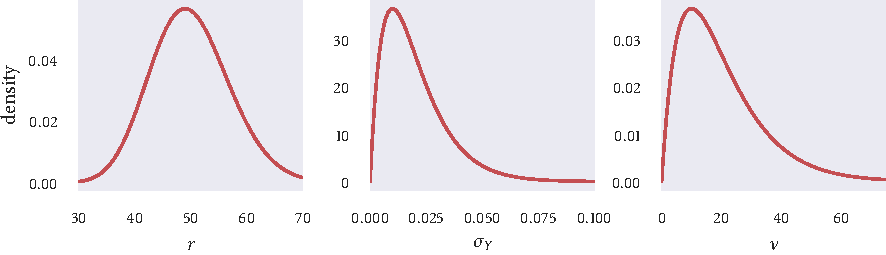
\includegraphics{vicsek_priors.pdf}
  \caption{Probability density functions representing our prior beliefs about plausible
    parameter values of the Vicsek model. These distributions represent
    weakly-informative priors, allowing a large range of possible parameter values.}
  \label{fig:vicsek_priors}
\end{figure}

Having specified the likelihood function, and quantified our prior beliefs about the model
parameters, we now have all the ingredients necessary to target the posterior.
Unfortunately, the discontinuity in the weighting function of the Vicsek model results in
a discontinuous posterior. As Stan requires a continuously differentiable posterior to
implement its NUTS algorithm, we instead target the posterior distribution with a random
walk Metropolis--Hastings sampler.

We implement the random walk sampler for $1,100,000$ iterations. The first $100,000$
iterations of the scheme are discarded to allow the sampler to converge.  The chains were
initialised as draws from our prior beliefs. The output of this scheme is summarised in
\cref{tab:vicsek_sim_study_summary}.

\cref{fig:vicsek_sim_study_chains} shows the chains generated by our inference scheme,
having discarded the initial burn-in period. From these trajectories we see evidence that
our sampler has converged: the chains oscillate around fixed values with common
variance.  The samples generated by these chains are visualised in
\cref{fig:vicsek_sim_study_hists}.  The true parameter values used to generate the data
are shown by vertical green lines. See that in each posterior the true value is
successfully captured by our posterior beliefs, and lies close to the posterior mode.
Moreover, our prior beliefs are overlain in red. Our prior beliefs appear flat in
comparison to our posteriors, reflecting that our beliefs have updated considerably in
light of the data.
\begin{table}[tbp]
  \begin{tabular}{@{}lrrrrr@{}}
    \toprule
    Parameter    & mean  & sd   & 5\%   & 95\%  & ESS     \\
    \midrule
    $r$          & 50.02 & 0.04 & 49.99 & 50.11 & 12\,290 \\
    $\sigma_{Y}$ & 0.03  & 0.00 & 0.03  & 0.03  & 44\,560 \\
    $\nu$        & 7.01  & 0.51 & 6.31  & 7.99  & 47\,420 \\
    \bottomrule
  \end{tabular}
  \caption{Summarising the posterior realisations for the parameters inferred in fitting
      the Vicsek model to simulated data. Realisations were made by implementing a random
      walk Metropolis--Hastings sampler. Columns report the posterior mean and standard
      deviation for each parameter. In addition to this, the fifth and ninety-fifth
  percentiles of our posteriors are quantified. Finally, the effective sample size of each
  chain is computed (and rounded to the nearest multiple of ten).}
  \label{tab:vicsek_sim_study_summary}
\end{table}
\begin{figure}[tbp]
  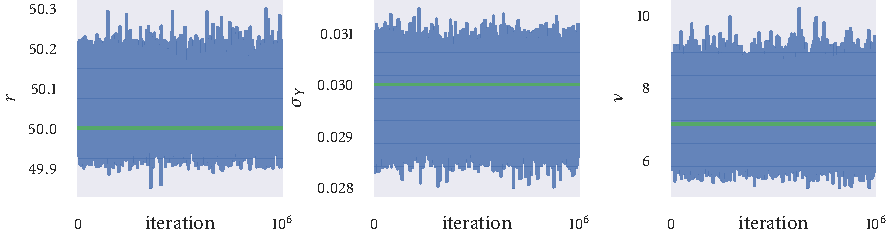
\includegraphics{mh_r_trace.pdf}
  \caption{Sequences of the random walk Metropolis--Hastings sampler for the Vicsek model.
      The initial $100,000$ iterations are discarded to allow a burn-in period. Horizontal
      green lines represent the true parameter values used to generate the simulated data.
      The chains look well-behaved, showing no irregularities, and suggest that our
  sampler has converged.}
  \label{fig:vicsek_sim_study_chains}
\end{figure}
\begin{figure}[tbp]
  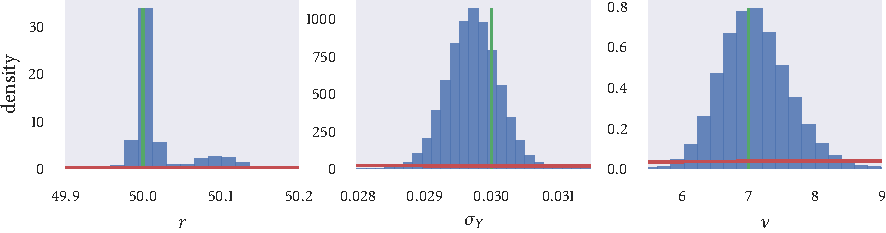
\includegraphics{mh_r_hist.pdf}
  \caption{Distributions of the samples realised from the posterior distribution. The
    green lines represent the known parameter values we seek to recover. Prior beliefs are
    overlain in red. Our posterior beliefs are seen to accurately capture the true
    parameter values. The data can be seen to have been very informative, as our posterior
    beliefs have updated considerably from our prior beliefs.}
  \label{fig:vicsek_sim_study_hists}
\end{figure}

Considering the output of this simulation study, we conclude that we can accurately
infer the true parameter values of data simulated from the Vicsek model. This gives us
confidence in moving forward to fit this model to real data.

\subsection{Continuous models}
\label{ssec:cont_models}

We have demonstrated that we can fit the Vicsek model to simulated data.  We now seek to
fit the power-law weighted (\cref{eq:power_law_interaction}) and Gaussian weighted
(\cref{eq:gaussian_interaction}) models to simulated data.

As these models implement continuous interaction rules, we may attempt parameter inference
using the Stan programming language. \cref{eq:likelihood} can be used to quantify the
likelihood of observing simulated data. To target the posterior we combine this likelihood
with our prior beliefs.

The power-law and Gaussian weighted models represent similar interaction rules. As with
the parameters $\nu$, $\sigma_Y$ and $r$, we shall use gamma distributions to quantify our
prior beliefs about $\alpha$ and $\sigma_X$.  To ensure that our prior beliefs between
these models are consistent, we shall determine our beliefs by considering plausible values
of the weighting $\omega_{ij,t}$. Using information about $d_{ij,t}$, along with
\cref{eq:power_law_interaction,eq:gaussian_interaction}, we can use our beliefs about
$\omega_{ij,t}$ to derive beliefs about $\alpha$ and $\sigma_X$.

To realise our prior beliefs we shall make two probabilistic statements about
$\omega_{ij,t}$. These can be used to determine prior distributions which best reflect
these statements. Firstly, we consider the weighting which agent $i$ gives to its closest
neighbour at time $t$. We believe with probability $0.025$ that this weighting will be less
than or equal to $0.25$. Similarly, we believe with probability $0.975$ that the
weighting which agent $i$ gives to its fifth closest neighbour will be less than or equal
to $0.90$.  More concisely, we can express these statements as:
\begin{align}
  \label{eq:omega_statements}
  \begin{split}
    P(\omega_{ij, t}({\min_j(d_{ij,t}, 1)}) \leq 0.25) & = 0.025, \\
    P(\omega_{ij, t}({\min_j(d_{ij,t}, 5)}) \leq 0.90) & = 0.975,
  \end{split}
\end{align}
where $\omega_{ij, t}({\min_j(d_{ij,t}, k)})$ is the influence of agent $i$'s $k$-th
closest neighbour at time $t$. To determine prior beliefs which best reflect these
statements, we seek shape and scale parameters for our gamma priors which minimise:
\begin{equation*}
  [P(\omega_{ij, t}({\min_j(d_{ij,t}, 1)}) \leq 0.25) - 0.025]^2
  + [P(\omega_{ij, t}({\min_j(d_{ij,t}, 5)}) \leq 0.90) - 0.975]^2.
\end{equation*}
A simple numerical optimisation routine can be used to minimise this function. With this
we realise prior beliefs:
\begin{align}
  \label{eq:gauss_power_priors}
  \begin{split}
    \alpha   & \sim \Ga(2, 2) \\
    \sigma_X & \sim \Ga(5, 5).
  \end{split}
\end{align}
\begin{figure}[tbp]
  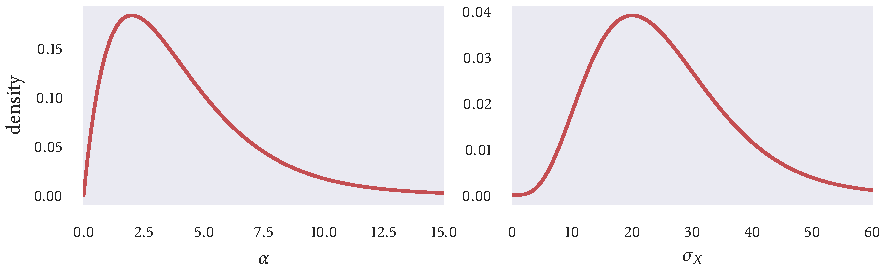
\includegraphics{gauss_power_priors.pdf}
  \caption{Probability density functions representing our prior beliefs about $\alpha$
    and $\sigma_X$, the interaction parameters of the power-law and Gaussian weighted
    models respectively. These prior beliefs are also given in
    \cref{eq:gauss_power_priors}.}
\end{figure}

\subsubsection{Power-law weighted}

The initial conditions for our simulated data are taken from an observation of a real
flocking event. A realistic-looking flock is generated with parameters $\alpha=1.5$,
$\sigma_Y=0.03$ and $\nu=7$.  \cref{fig:power_sim_study} shows the trajectories realised
by this simulation. We then seek to recover the known parameter values by inference.
\begin{figure}[tbp]
  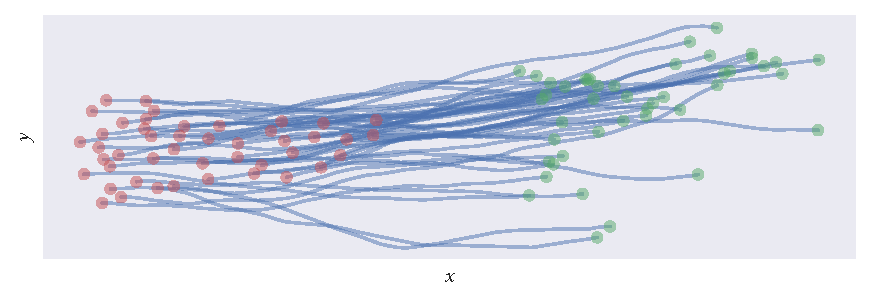
\includegraphics{power_sim.pdf}
  \caption{Simulated data generated by a run of the power-law weighted model with
    parameter values $\alpha=1.5$, $\sigma_Y=0.03$ and $\nu=7$. The data represents the
    trajectories of motion of $N=45$ agents moving for $200$ frames. Initial conditions
    for this simulation were realised from an observation of a real flocking event.}
  \label{fig:power_sim_study}
\end{figure}

Stan is used to perform parameter inference on this model. Four independent chains are
initialised as realisations from our prior beliefs. Each chain is then simulated for
$10,000$ iterations, with the first $5000$ iterations discarded to allow a warm-up period.
\cref{tab:power_sim_study_summary} summarises the posterior draws generated by this run. 
The tabulated split-$\widehat{R}$ values indicate that our sampler has converged for all
parameter values.  

The chains generated by this sampler are shown in \cref{fig:power_sim_study_chains}. Each
colour represents an independent chain.  See that although the four chains were
initialised at different locations, they all converge to the same region.

Histograms of our posterior draws are presented in \cref{fig:power_sim_study_hists}. The
vertical green lines in these plots represent the true parameter values. In each case, our
posteriors can be seen to capture the true values. In fact, the true parameter values are
seen to be well represented by the posterior mode. Our prior beliefs are overlain in red.
These priors appear flat in comparison to our posteriors, indicating that we have learnt a
from the data.

\begin{table}[p]
  \begin{tabular}{@{}lrrrrrr@{}}
    \toprule
    Parameter    & mean  & sd   & 5\%  & 95\% & ESS                & $\widehat{R}$ \\
    \midrule
    $\alpha$     & 1.50  & 0.02 & 1.48 & 1.54 & 13\,130            & 1.0           \\
    $\sigma_{Y}$ & 0.03  & 0.00 & 0.03 & 0.03 & 11\,400            & 1.0           \\
    $\nu$        & 7.09  & 0.50 & 6.28 & 7.91 & 11\,580            & 1.0           \\
    \bottomrule
  \end{tabular}
  \caption{Summarising the posterior realisations made by Stan. Each row represents a
      parameter of the power-law weighted model, and our posterior beliefs about it.
      Columns show the posterior mean and standard deviation of each parameter, along with
      the fifth and ninety-fifth percentiles of our beliefs. The number of effective
      samples drawn from the posterior is quantified by ESS. The values of
      $\widehat{R}$ computed indicate that our chains have converged.}
  \label{tab:power_sim_study_summary}
\end{table}
\begin{figure}[p]
  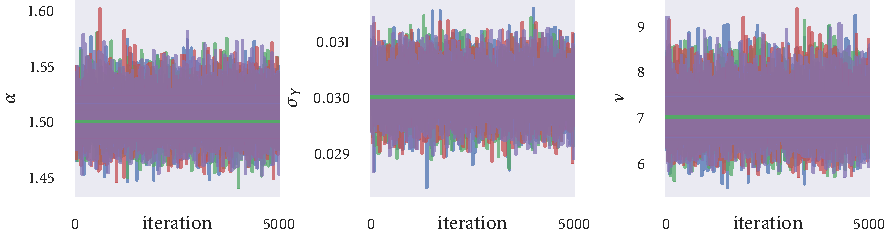
\includegraphics{stan_power_trace.pdf}
  \caption{Trajectories of the four independent chains for each parameter
      value. Each chain is overlaid in a different colour. Although each chain
      was initialised at a different starting point, they can be seen to
      converge to the same distribution. Chains were simulated for $10,000$
      iterations, with the first $5000$ iterations discarded to allow convergence.
      The chains can be seen to oscillate around the true parameter values,
      represented by the green horizontal lines.}
  \label{fig:power_sim_study_chains}
\end{figure}
\begin{figure}[p]
  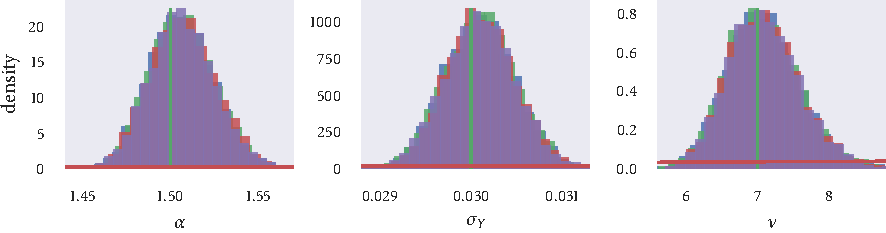
\includegraphics{stan_power_hist.pdf}
  \caption{Histogram plots of our samples drawn from the posterior distribution. The true
  parameter values are represented by the green vertical lines. See that the true value
  for each parameter is well represented by the posterior mode. Prior beliefs are overlain
  in red.}
  \label{fig:power_sim_study_hists}
\end{figure}

\subsubsection{Gaussian weighted}

As with the previous simulation studies, we forward simulate this model with $N=45$ agents
and $T=200$ time steps, using initial conditions from a real flocking event.
\cref{fig:gauss_sim_study} illustrates the data generated by this simulation. Here,
parameters $\sigma_X=20$, $\sigma_Y=0.025$ and $\nu=7$ were used to produce
realistic-looking flocking behaviour.

Here we shall use Stan to perform parameter inference. Four independent sequences are
initialised at draws from our prior beliefs and simulated for $10,000$ iterations. The
first $5000$ iterations are discarded to allow for a warm-up period.
\cref{tab:gauss_sim_study_summary} summarises the output from this run.  The reported
split-$\widehat{R}$ values indicate that the sequences have converged. 

The output visualised in \cref{fig:gauss_sim_study_chains,fig:gauss_sim_study_hists} shows
a well-behaved sampler, capable of capturing the true parameter values of the power-law
weighted model from simulated data.

\begin{figure}[tbp]
  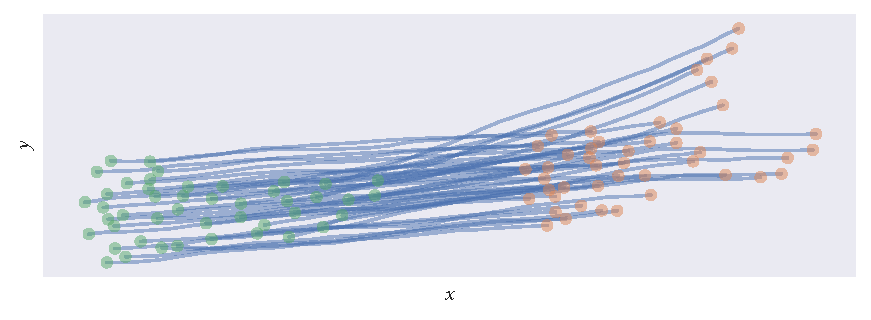
\includegraphics{gauss_sim.pdf}
  \caption{Data generated from a simulation of the Gaussian weighted model with
  parameters $\sigma_X=20$, $\sigma_Y=0.025$ and $\nu=7$. Initial conditions are taken
  from an observation of a real flocking event.}
  \label{fig:gauss_sim_study}
\end{figure}
\begin{table}[tbp]
  \begin{tabular}{@{}lrrrrrr@{}}
    \toprule
    Parameter    & mean   & sd   & 5\%    & 95\%    & ESS                & $\widehat{R}$ \\
    \midrule
    $\sigma_{X}$ & 19.94 & 0.20  & 19.60  & 20.27   & 13\,310            & 1.0           \\
    $\sigma_{Y}$ & 0.025 & 0.00  & 0.024  & 0.025   & 11\,700            & 1.0           \\
    $\nu$        & 7.25  & 0.53  & 6.41   & 8.12    & 11\,360            & 1.0           \\
    \bottomrule
  \end{tabular}
  \caption{Summaries of our posterior beliefs realised in fitting the Gaussian weighted
  model to simulated data. Each row represents a parameter of the Gaussian model. Each
  column presents a different summary of our posterior beliefs.}
  \label{tab:gauss_sim_study_summary}
\end{table}
\begin{figure}[tbp]
  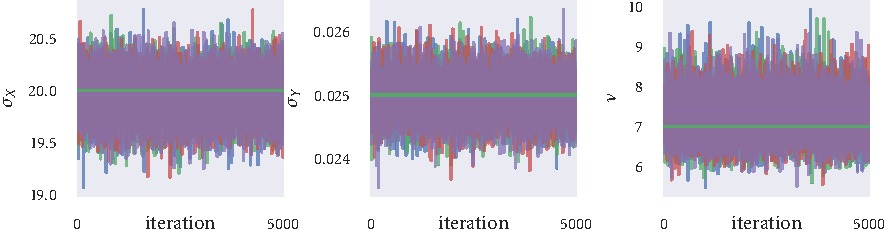
\includegraphics{stan_gauss_trace.pdf}
  \caption{Visualising the Markov chains generated by Stan's NUTS algorithm. Each colour
  represents an independent chain. Although the chains are initialised as different draws
  from our priors, they all converge to some common distribution.}
  \label{fig:gauss_sim_study_chains}
\end{figure}
\begin{figure}[tbp]
  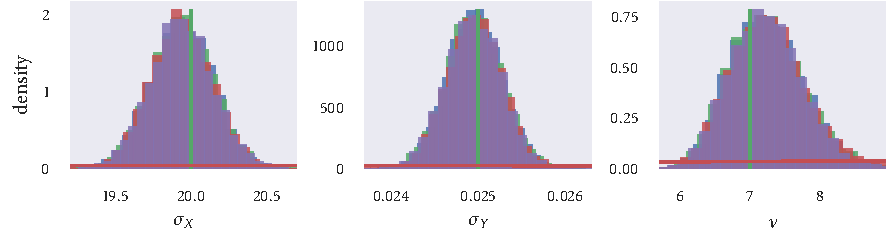
\includegraphics{stan_gauss_hist.pdf}
  \caption{Draws realised by Stan in fitting the Gaussian weighted model to simulated
  data. The true values (green vertical lines) are well represented by our posterior
  beliefs. Our posterior beliefs have updated considerably from our prior beliefs
  (red).}
  \label{fig:gauss_sim_study_hists}
\end{figure}

\subsection{Topological model}

In \cref{ssec:cont_models} we demonstrated that it is possible to accurately capture the
parameters of the power-law and Gaussian weighted models from simulated data. However, we
are interested in comparing the predictive-performance of metric and topological models
with real data. As such, we also desire to perform a simulation study on our topological
model.

\cref{eq:likelihood,eq:top_interaction} allow us to quantify the goodness of fit of the
topological model with parameters $k$, $\sigma_Y$ and $\nu$ to observations of a flocking
event. To target the posterior we must combine this likelihood with prior beliefs about
the model parameters. We have no reason to believe that the noise experienced by
individuals under a topological regime would be any different to that experienced under a
metric regime. As such, our prior beliefs about the noise parameters $\sigma_Y$ and $\nu$
shall remain the same as in the metric case: as expressed in \cref{eq:vicsek_priors}.

We are then left to quantify our prior beliefs about $k$, the number of nearest neighbours
which an agent interacts with. Previous work suggested that agents interact with their
closest six to seven nearest neighbours \parencite{ballerini08}. However, this work
investigated flocking events which took place in three spatial dimensions. As we are
focussing on data restricted to a two-dimensional plane, we believe that the number of
nearest neighbours will be lower than six to seven. We find that a $\Ga(6, 1/2)$
distribution captures a wide range of plausible values for $k$ (\cref{fig:top_priors}).

The topological model is forward simulated to generate data for the simulation study.
Forty-five agents are simulated for two-hundred time steps. Each agent interacts with its
closest $k=3$ nearest neighbours. Noise was generated from a generalised Student's
$t$-distribution with scale $\sigma_Y=0.03$ and degrees of freedom $\nu=7$.

\begin{figure}[tbp]
    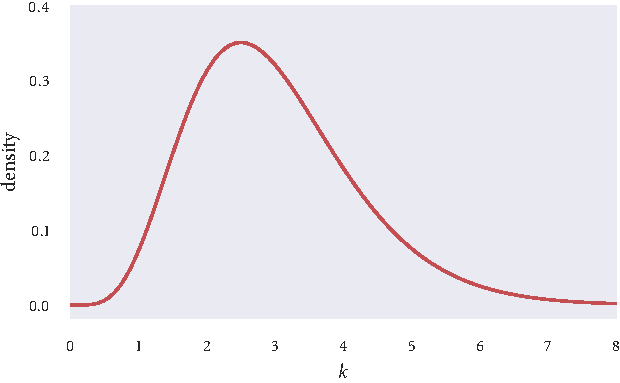
\includegraphics{top_priors.pdf}
    \caption{Prior beliefs about the number of nearest neighbours $k$ which an agent
    interacts with, expressed by a $\Ga(6, 1/2)$ distribution.}
    \label{fig:top_priors}
\end{figure}

\begin{figure}[tbp]
    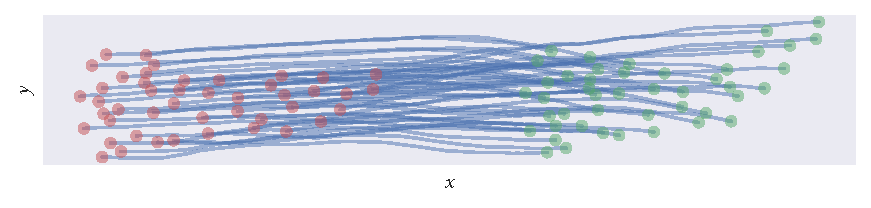
\includegraphics{top_sim.pdf}
    \caption{Data used for our simulation study of the topological model. Each agent was
    simulated to interact with its nearest $k=3$ neighbours, and was subject to noise
    generated from a generalised Student's $t$-distribution with location $0$, scale
    $\sigma_Y=0.03$ and degrees of freedom $\nu=7$.}
    \label{fig:top_sim}
\end{figure}

\begin{table}[tbp]
\begin{tabular}{@{}lrrrrrr@{}}
\toprule
Parameter & mean &    sd & 5\% & 95\% & ESS & $\widehat{R}$ \\
\midrule
$k$ & 2.98 & 0.02 &   2.94 &    3.02 &            16\,710 &       1.0 \\
$\sigma_{Y}$ & 0.03 & 0.0 &   0.03 &    0.03 &            13\,240 &       1.0 \\
$\nu$ & 7.04 & 0.50 &   6.20 &     7.81 &            13\,355 &       1.0 \\
\bottomrule
\end{tabular}
\caption{Summarising samples drawn from the posterior distribution by Stan's
implementation of the No-U-Turn-Sampler. Each row represents a parameter of the
topological model.} 
\end{table}

\begin{figure}[tbp]
    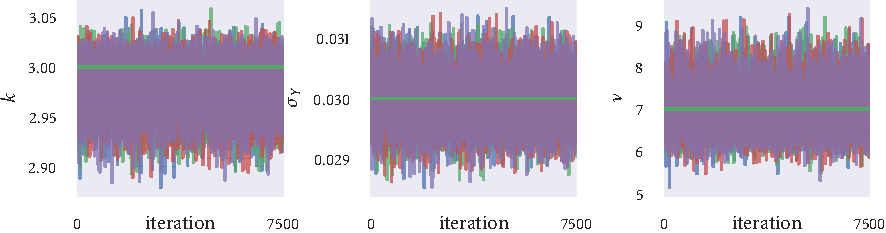
\includegraphics{stan_top_trace.pdf}
    \caption{Four independent sequences generated by the NUTS algorithm.}
\end{figure}

\begin{figure}[tbp]
    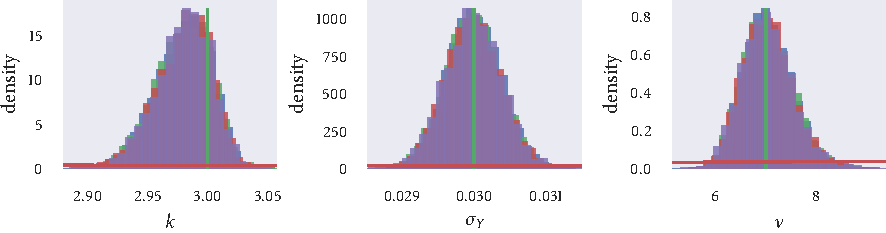
\includegraphics{stan_top_hist.pdf}
    \caption{}
\end{figure}

\section{Hierarchical models}

Hierarchical models represent a more demanding inference problem owing to the increased
number of model parameters to infer. The simulation studies performed in
\cref{sec:glob_mod} required three parameters to be inferred per model: one interaction
parameter and two noise parameters. In the hierarchical models introduced in
\cref{ssec:hier_mod} each agent has its own interaction parameter, as well as its own
scale for the generalised Student's $t$-distribution. With this, to fit a hierarchical
model to data describing the movements of $N$ individuals we are required to infer $2N+1$
parameters and $4$ hyperparameters.



